
\section{B2}

\subsection{B2.1}

\subsubsection{a}

%I = [n, m], 0 <= n <= m <= inf., n, m \in N.
%Path is s0s1s2s3...sns{n+1}s(n+2}...
%For i = 0..n-1, M, s_i |= \Phi_1,
%and exists j such that k = n..j-1 M, s_j |= \Phi_1, and M, s_m |= \Phi_2

$\sigma = s_0 s_1 s_2 ..$.

$\sigma \models \Phi_1 U^I \Phi_2$ if and only if there exists a $j$
such that:

$j \in I$

$s_j \models \Phi_2$

For all $i$ given by $0 \leq i < j$: $s_i \models \Phi_1$.

\subsubsection{b}

Case $[0, \infty)$: $\Phi_1 U \Phi_2$.

Case $[0, n]$: $\Phi_1 U^{\leq n} \Phi_2$.

$[n, \infty)$ and $[n, m]$ would require that the paths obey $\Phi_1$
along the path until $n$, and after $n$ steps, another condition must hold.
But there is no way to describe something after at least $n$ steps,
only at most $n$ steps.

\subsubsection{c}

An alternative to the P state operator, named Q,
that have four operands instead of two.
It has the normal interval and path operands,
but it also has a step and state formula operands.
The Q operator requires that for a path to hold that the state formula holds
for the first $n$ states, and then the path formula
must hold from the $n+1$ state.
$n$ must be at least 1.
It would look something like $Q_{J,n, \Phi} [\phi]$.

This is the way it would be used to encode the new until:

$Q_{J, n, \Phi_1} [\Phi_1 U \Phi_2]$

\subsubsection{d}

First we get the probability matrix of going from each state to
some state using exactly $n$ steps,
and only using states that satisfies $\Phi_1$.
To get this, we modify the transition system such that states that does not satisfy
$\Phi_1$ only have self-loops to themselves.

After that, we find the probability of each state satisfying $\Phi_1 U \Phi_2$.
And then, to find the probability that a state $s_i$ satisfies $\Phi_1 U^{\geq n} \Phi_2$,
we simply multiply each of the probabilities of going from $s_i$ to $s_j$ for all $j$ with
the probability that $s_j$ satisfies $\Phi_1 U \Phi_2$, and sum the resulting terms.

\subsection{B2.2}

\subsubsection{a}

The coarsest probabilistic bisimulation relation is:

$R \subseteq S \times S = \{\{s_0s_0\}, \{s_1s_1\}, \{s_1s_4\}, \{s_2s_2\}, \{s_3s_3\}, \{s_4s_1\}, \{s_4s_4\}, \{s_5s_5\}\}$

\subsubsection{b}

$M/\sim$

\begin{figure}[!htb]
\centering
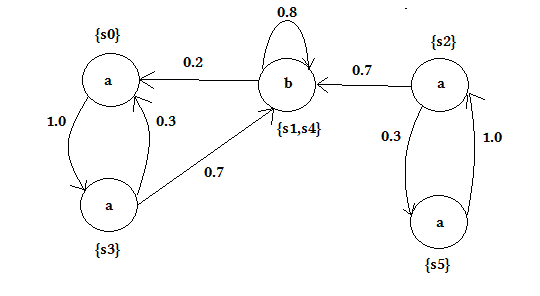
\includegraphics{images/bisimulation}
\caption{Bisimulation quotient}
\end{figure}

\subsubsection{c}
The relationship between the steady state distribution of $M$ and that of bisimulation quotient $M/\sim$ of $M$ is:

$\forall T. \sum_{s_i \in T} \pi(i)=\pi(T)$

Where $T$ is an equivalence class

\subsubsection{d}
If we were to choose a different labelling function $L$ for the DTMC $M$ giving the coarsest possible probabilistic bisimulation, then $L$ should give the same label to all states.
This however means that there's no difference between the states.

\subsubsection{e}
Equivalence classes of a probabilistic bisimulation constitutes partioning. We know from the definition for bisimulation relations that for each pair of states, where each state belongs to the same
equivalance class, it holds that:

$P(s1,T)=P(s2,T)$

and this is the same as lumpability.

\subsubsection{f}
Since lumpability in this case implies bisumulation quivalence, then it is not possible. Then according to theorem 10.67 that PCTL* cannot distinguish between two states that belongs to the same partion.
Lumpability in this case implies bisimulation equivalence because the two definitions of 10.60 are satisfied.

